\section{Experiments and Analysis}
\label{sec:experiments_analysis}

We conduct an evaluation of several MID methods based on BlendX, as well as the original MixX. 

\paragraph{Methods} 
In recent years, the joint learning of intent-detection and slot filling has emerged as the \textit{de facto} standard for these tasks.
Given the MixX framework's dual provision of multi-intent and slot information for each utterance, this trend has similarly permeated MID research. \cite{Cheng_2023,Tu_2023,chen-etal-2022-transformer,xing-tsang-2022-co,9747843,qin-etal-2021-gl,jiang-etal-2023-spm}
However, given that our emphasis in this study is solely on (multi-)intent detection, we make modest modifications to the two most predominant supervised methods to suit our objective:
\begin{itemize}
    \item \textbf{TFMN} \cite{chen-etal-2022-transformer,Cheng_2023}: 
    This approach first predicts the number of intents, denoted as $k$, in a multi-intent utterance. 
    Subsequently, it yields the top-$k$ options based on the predicted probability distribution.
    We used a variant of the original TFMN method that considers only utterance-level supervision instead of token-level, as annotating utterances from the Generative approach with token-level labels is challenging.\footnote{Since we focus on (multi-)intent detection, we find it reasonable to consider only sentence-level supervision.}
    \item \textbf{SLIM} \cite{9747477}: 
    This method decomposes multi-label classification into a series of binary classifications. 
    Specifically, it gauges the likelihood of each intent using the \texttt{sigmoid} function and then collects the intents whose probability exceeds a given threshold.
\end{itemize}

Furthermore, we also adopt ChatGPT (\texttt{gpt-3.5-turbo-0613}) as an extra baseline.
Figure \ref{figure:prompt_chatgpt_figure} illustrates how we design prompts for facilitating in-context learning for MID.
Note that the utilization of ChatGPT contrasts with the predominantly supervised fine-tuning approaches.
This sheds light on the potential of generative approaches to tackle MID with little to no examples provided.

\begin{figure}[t]
    \setlength{\fboxsep}{7pt} 
    \noindent\fbox{%
        \begin{minipage}{\dimexpr\columnwidth-2\fboxsep-2\fboxrule\relax}
        
            \fontsize{9pt}{11pt}\selectfont 
            \setlength{\parskip}{5pt} 
            \textbf{Instructions:} \textsc{You are an Intent Detection Model on single utterance. Detect single or more intent(s) of each utterance UP TO 3.} \\\vspace{-5pt}
            
            \textbf{Example: } \textsc{[$k$ pairs of a multi-intent utterance and its corresponding intents]} \\\vspace{-5pt}

            \textbf{Query: } \textsc{[query]} \\\vspace{-5pt}
            
            \textbf{Answer: } \textsc{[answer]}           
               
        \end{minipage}%
    }
    \caption{Prompt design for solving MID with in-context learning. 
    We employ the few-shot setting where $k$ multi-intent utterances are provided, each associated with up to three intents. 
    The \textsc{[Answer]} part is filled in to predict the intent of \textsc{[Query]}. 
    Appendix \ref{subsec:prompt_evaluate} presents detailed illustrations.}
    \label{figure:prompt_chatgpt_figure}
\end{figure}

\begin{table*}
    \scriptsize
    \centering
    \extrarowheight=\aboverulesep
    \addtolength{\extrarowheight}{\belowrulesep}
    \aboverulesep=0pt
    \belowrulesep=0pt
    \begin{tabular}{caaccccc}
        \toprule
            \multirow{2}{*}{\shortstack[c]{\textbf{Model}}} & \multicolumn{2}{a}{\textbf{Split}} & \multicolumn{4}{c}{\textbf{Dataset (Metric: Accuracy)}} \\
            & \textbf{Training} & \textbf{Test} & \textbf{SNIPS} & \textbf{ATIS} & \textbf{Banking77} & \textbf{CLINC150}\\
        \midrule
        \multirow{3}{*}{\shortstack[c]{TFMN}} & MixX & MixX & 95.68* $\pm 0.57$ & 77.98* $\pm 0.57$ & 76.61 $\pm 1.17$ & 85.88 $\pm 1.03$ \\
        & MixX & BlendX & 52.51 $\pm 1.86$ & 42.51 $\pm 1.48$ & 37.31 $\pm 0.81$ & 42.45 $\pm 2.40$ \\
        & BlendX & BlendX & 94.93 $\pm 0.85$ & 76.50 $\pm 0.83$ & 63.99 $\pm 0.81$ & 77.96 $\pm 0.82$ \\ 
        \midrule
            \multirow{3}{*}{\shortstack[c]{SLIM}} & MixX & MixX & 95.97* $\pm 0.23$ & 77.10* $\pm 0.28$ &  83.71 $\pm 0.88$ & 88.67 $\pm 0.56$ \\
            & MixX & BlendX & 93.51 $\pm 0.18$ & 72.80 $\pm 1.48$ &  69.89 $\pm 0.46$ & 73.39 $\pm 2.46$ \\
            & BlendX & BlendX & 95.73 $\pm 0.86$ & 76.92 $\pm 0.84$ & 75.30 $\pm 0.71$ & 85.62 $\pm 0.51$ \\ 
        \midrule
            \multirow{2}{*}{\shortstack[c]{gpt-3.5-turbo}} & - & MixX & 81.68 & 40.30 & 30.90 & 49.22 \\
            & - & BlendX & 76.18 & 38.84 & 22.67 & 37.55 \\
        \bottomrule 
    \end{tabular}
    \caption{
    Evaluation of three competitive MID models on MixX and BlendX.
    The reported numbers represent the averages and standard deviations from five distinct executions.
    The symbol $*$ indicates numbers derived from our re-implementation, where we have specifically excluded joint learning with slot filling.
    }
    \label{table:table_main}
    \centering
\end{table*}

\paragraph{Results} 
The main results are listed in Table \ref{table:table_main}. 
First, we reaffirm the widely recognized observation that current supervised methods show reasonable performance when both trained and evaluated with MixX.
Yet, the narrative shifts significantly when these models are evaluated on our new datasets.
In this configuration (training: MixX \& test: BlendX), where the test data distribution deviates from the training distribution, every model shows a significant performance drop, with some declining by up to 40\%.
This outcome suggests that the original MixX may lack the complexity required to comprehensively evaluate the abilities of MID methods.

On the other hand, while transitioning the training data from MixX to BlendX does lead to some performance recovery on the test set, the results do not match the original performance observed when evaluated on MixX. 
This implies that BlendX intrinsically possesses greater complexity, making it more challenging to master.

Additionally, we find that ChatGPT's performance on MID datasets is subpar. 
This indicates that despite ChatGPT's adaptability, more work is needed to optimize its application for this task.

\begin{figure}[t]
\begin{center}
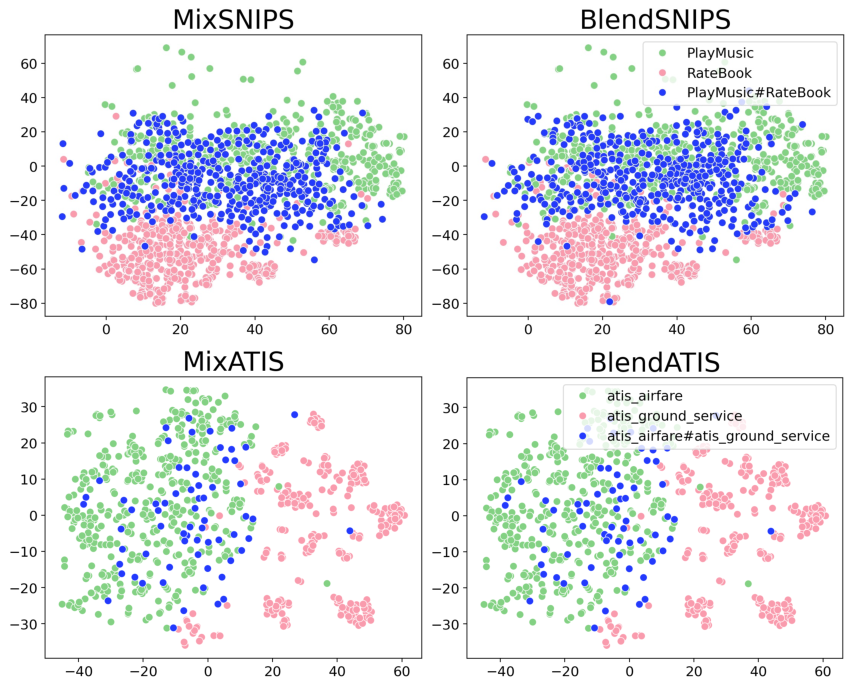
\includegraphics[scale=0.53]{images/Visualization9.pdf} 
\caption{Visualization of MixX (Left) and BlendX (Right) in the $\mathbb{R}^2$ space (datasets: SNIPS, ATIS).}
\label{fig:visualization}
\end{center}
\end{figure}

\paragraph{Visualization}
Figure \ref{fig:visualization} shows data samples from SNIPS and ATIS. 
They are embedded with SBERT and projected into a 2-dimensional space via t-SNE.
In the upper part of the figure, the green and pink dots correspond to utterances whose intents are \texttt{PlayMusic} and \texttt{RateBook}, respectively. 
Meanwhile, the blue dots represent multi-intent utterances with \texttt{PlayMusic\#RateBook}, sourced from MixSNIPS and BlendSNIPS.
The two graphs show nearly identical distributions, implying that although BlendX utterances are expected to be more diverse and noisy, they still occupy a space where data points capture the semantics of both intents.

\begin{table}[t]
\scriptsize
\centering
\extrarowheight=\aboverulesep
\addtolength{\extrarowheight}{\belowrulesep}
\aboverulesep=0pt
\belowrulesep=0pt
    \begin{tabular}{a c c c c}
        \toprule
            \textbf{Data Split} & \multicolumn{4}{c}{\textbf{Testset: BlendX (Metric: Accuracy)}} \\
            \textbf{Generated By} & \textbf{SNIPS} & \textbf{ATIS}& \textbf{Banking77}& \textbf{CLINC150} \\
        \midrule
            Na\"ive & 95.32 & 73.23 & 62.30 & 80.73 \\
            Manual & 25.32 & 42.40 & 8.05 & 25.73 \\
            Generative & 81.58 & 53.93 & 27.95 & 60.17 \\
        \bottomrule
    \end{tabular}
\caption{
Experiments with different subsets of BlendX, grouping data instances by the method used for their creation.
TFMN, trained with MixX, is evaluated on these subsets. 
It is observed that the Manual method contributes the most complexity and difficulty to BlendX.
}
\label{table:ablation_study}
\centering
\end{table}

\paragraph{Ablation study for concatenation methods}
To evaluate the impact of different merging methods within BlendX, we categorize subsets based on the concatenation approach and measured their accuracy using TFMN. 
These results are presented in Table \ref{table:ablation_study}. 
We observe that the subset generated by Manual is consistently more complex than the one created using the Na\"ive method. 
Comparatively, the subset merged via the Generative approach displays greater complexity than the case of Na\"ive but is less intricate than the case of Manual approach. 
These findings indicate that the Manual approach is a highly effective method of construction, facilitating both explicit and implicit concatenation. 
On the other hand, the Generative method tends to yield utterances akin to explicit concatenation, albeit with occasional instances of creativity.